% Please do not change the document class
\documentclass{scrartcl}

% Please do not change these packages
\usepackage[hidelinks]{hyperref}
\usepackage[none]{hyphenat}
\usepackage{setspace}
\usepackage{graphicx}
\usepackage{subcaption}
\doublespace

% You may add additional packages here
\usepackage{amsmath}

% Please include a clear, concise, and descriptive title
\title{When should Game Developers use Vertex Shader Animations over Skeletal Animations?}

% Please do not change the subtitle
\subtitle{COMP130 - Software Engineering}

% Please put your student number in the author field
\author{1703086}

\begin{document}

\maketitle

\abstract{This essay will be comparing two popular animation techniques and reviewing how vertex animation could be used as a better creative and cheaper alternative to skeletal animation, while looking at games that used Vertex animation in those ways.}
%things to include today: LOD level of detail, mention abzu art style, collisions for Vertex shaders, conclusion talk about styleized animations, GPU vs CPU talk

\section{Introduction}
Animation is an integral part of video games and over the years there has been lots of advancements in how animation is created for games, there are now many different ways animation techniques that can be done in games these days.
\\~\\
This essay will be looking at 2 popular 3D animation techniques used in games development, and will be comparing the two to find out when and why each animation technique should be used depending on what needs to be animated.
\\~\\
This essay will also will review and look at cases in which vertex animation was used as a better and cheaper alternative to animating game objects that would normally be animated using skeletal animation.

%Quickly introduce the vertex and skeletal animations techniques and describe why you want to compare them for games development and what benefit this will be to game developers.

\section{Vertex shader VS Skeletal}

\subsection{Quick overview on what Vertex shader and Skeletal animations are}
\textbf{Skeletal animation} is the process of animating a mesh that is skin weighted to an armature or bone rig, the process is most oftenly done in animation software such as Maya or Blender.
Skeletal animation is also a type of vertex shader, so it can work hand in hand with other shaders, but alone it is fairly limited.\cite{ten}
Skeletal animation works by tweening/blending between different poses (keyframes) set at different times of the animation, the action of tweening/blending generates the other poses between the keyframes, filling in the animation with every single keyframed pose needed to create the illusion of animated movement.
\\~\\
\textbf{Vertex shader animation} is the process of animating a mesh with the use of applying a shader script. Shaders are a programmable part of the graphics pipeline and are created with the use of shading languages such as OpenGL's shading language GLSL or DirectX's High-Level Shader Language HLSL.\cite{twelve}
The way a vertex shader works is that it modifies the mesh it is applied to during the rendering pipeline; it transforms each individual vertices of the mesh per rendered frame creating the illusion of animated movement.\cite{nine}

\subsection{What is each animation technique best for?}
\textbf{Skeletal animation} is most commonly used to animate characters and creatures as it allows for precise control over a character's different body parts and apparel, it is also used for animating very specific set of movements for an object, such as a robotic arm or a tree.\cite{ten}
\\~\\
\textbf{Vertex shader animation} is most commonly used for animating special effects for game objects or for animating the movement of environmental objects such as grass, leaves, bushes, flames, water...ect.\cite{two}\cite{three}\cite{four}\cite{six}
Vertex shaders can be very extensive in their use as they can be programmed in many different ways.
\\~\\
An animation technique that can be done with Vertex shaders is Blendshapes (also known as morph target animation) which is the process of taking the vertex data of a mesh in two different poses, and then lerping their vertex positions over delta-time to perform the animation, this is essentially what skeletal animation is, just without the bones/joints and skin weighting.
Blendshapes are a great way for creating more specific animations with the use of vertex shaders.

\subsection{Comparing the two techniques}
Comparing these two animation techniques comes down to convenience, Vertex shaders are very inconvenient for creating complex locomotion types of animation for characters as they aren't built to handle precise movement to transform specific vertex areas of a mesh, but they are very convenient when it comes to transforming all the vertices of a mesh at the same time, like creating a wave effect on a mesh plain to make it look like ocean waves or a flag in the wind.
\\~\\
As for skeletal animation it is most convenient for creating very specific character or object movement animations like locomotion cycles, fighting move sets, interactions...ect but skeletal animation is quite inconvenient for creating general purpose animations that can act on more than one mesh/gameobject as they are animated around a specific armature rig, it is also inconvenient for creating animations that affect all areas of the mesh as the mesh is specifically skin weighted to certain bones of the rig.

%Outline the main differences between the 2 techniques and talk about how they are mainly each used in games. Compare how they could be used for the same animations on certain types of objects/meshes. Talk about how skeletal animation causes problems that vertex shaders can solve. 2 most common shading languages: OpenGL shading language GLSL and DirectX High-Level Shader Language HLSL. Things to mention: vertex Shaders, The graphics pipeline, LOD level of detail

\subsection{Skeletal animation used alongside Vertex shaders}
Because Skeletal animation is just a form of a vertex shader, Skeletal animation and vertex shader animation can work well alongside to make animated characters with interesting visual effects.
\\~\\
An example of this being done for a in-game character are these fictional creatures shown in this gif (https://i.imgur.com/U40e9Bm.gif) and in Figure 1 below, their main bodies are animated with skeletal animation but their cloud tails have a vertex shader applied to them to give them the continuous puffing up and down effect.
\\~\\
Game developers might also want to consider using Vertex shaders animations alongside Skeletal animations in order to come up with more visually interesting animations, such examples could be a slime monster, who's skin (mesh) is constantly moving around creating a bubbly slimy effect, while the main body of the monster is animated using bones.
\\~\\
\begin{figure}[h!]
  \centering
  \begin{subfigure}[b]{0.4\linewidth}
    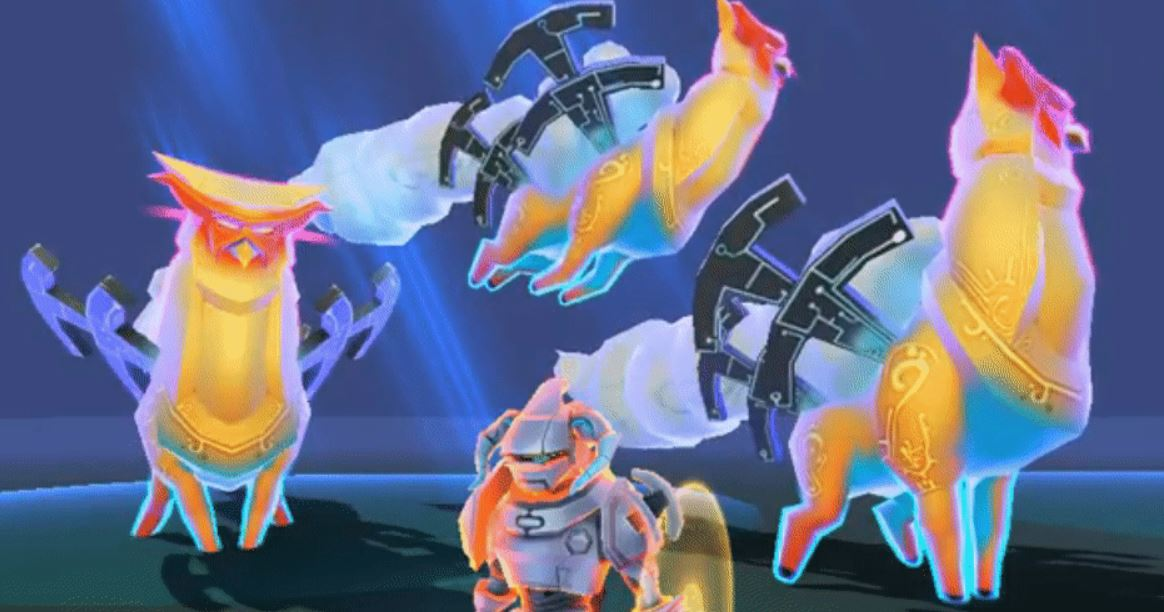
\includegraphics[width=\linewidth]{Capture1.jpg}
    \caption{Capture 1}
  \end{subfigure}
  \begin{subfigure}[b]{0.4\linewidth}
    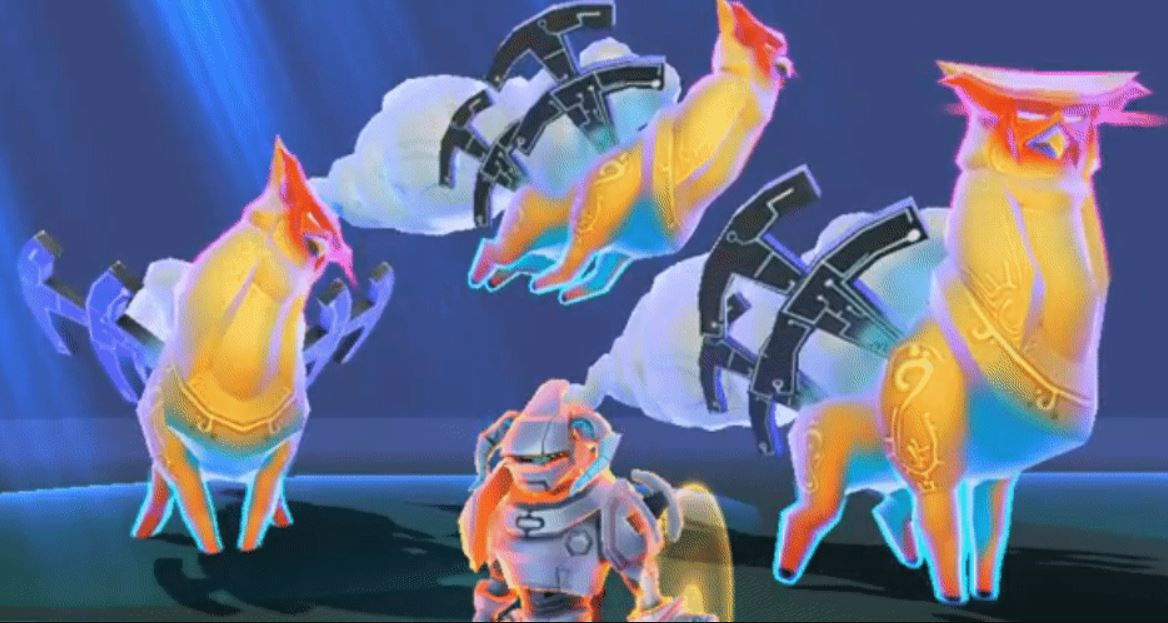
\includegraphics[width=\linewidth]{Capture2.jpg}
    \caption{Capture 2}
  \end{subfigure}
  \caption{Screen captures of the animated creatures}
  \label{fig:anim}
\end{figure}

\section{Cases in which vertex shader animations were a better solution to skeletal animations}

\subsection{Abzu}
The game Abzu (a game about swimming around in the ocean with lots of fish) had some very creative and innovative ways of animating their fish in order to save performance all while keeping high quality animations.
\\~\\
One of the lead developers of Abzu did a GDC talk about their technical art challenges and how they solved them.\cite{seven} One of their key challenges was trying to render over 10,000 animated interactive fish on screen at the same time, the big issue they had was animating the fish with skeletal animation, each fish had their own skeletal rig with about 60 to 100 joints and updating each fish every frame with 10,000 fish on screen meant they had to update around 1,000,000 joints per frame which would be extremely costly for processing wise. So their solution was Static mesh instancing with the use of vertex shaders and blendshapes.
\\~\\
So instead of using skeletal animation to animate swim cycles for the fish they wrote vertex shader scripts that allowed them to animate the fish using a mix of yaw rotations, sin waves and pans to transform the position of all the vertices of the mesh and distort it to look as if the fish is swimming. Because they animated the fish without bones means they were able to successfully render over 10,000 fish on screen without losing performance or frame-rate.
\\~\\
They also used vertex shader blendshape animation for some simple creature animations. Using this technique they could create animations such as biting animations for predator fish, by using the fish's mesh in a open mouth positions and a closed mouth position they could blend between the two poses creating the blendshape animation.\\
They managed to use this for crab walk cycles and seagull flying cycles all without the use of bones in engine to save performance.

\subsection{Fortnite}
The developers on Fortnite (a battle royal game with a focus on building mechanics and a cartoony art style developed by Epic Games) created some interesting ways of creating complex animations with vertex shaders to create culling animations, environment destruction animations and building block placement animations.
\\~\\
A Technical artist who worked on developing vertex animations did a GDC talk about the challenges and solution they found when creating certain animations for Fortnite.\cite{thirteen} The game has a very cartoony stylized look that they really wanted to incorporate into their animations, so they decided to use vertex shaders to create exaggerated cartoony wobble and bounce animations for their environmental objects, when certain objects and buildings are hit by the player they wobble and bounce to show the impact of the player. Vertex shaders are ideal for this kind of animation use, in contrast to skeletal animation, it is a lot easier to animate a bunch of vertices to wobble and bounce along a programmed mathematical equation then it would be to animate it by hand.
\\~\\
They also wanted to create a very stylized culling effect (culling in games is the process of rendering/showing or not rendering/hiding what is in the view of the player) to add to the overall exaggerated catoony style of the game. They used Vertex shaders to animated the process of making an environmental object being culled by making it pop up out of the ground with a slight bouncing effect to it. They did this by using a scale operation from the pivot point of the model. It was done with vertex shaders instead of updating the model's transform to scale it upwards, which would of been much more expensive to update on tick (per frame).
\\~\\
Placing down building blocks was explained to be a very difficult animation to create with Vertex shaders, it had been created with the use of skeletal animation techniques but was too performance heavy for what it should be and that's why they opted for using vertex shaders. An example of the animation of a building block wall in Figure 2 below. Their main problem was that you can't have access to the transform of subobjects (wooden board for example) using vertex shaders, so their solution was to create custom tools to get the data of each subobject separately in 3D modelling and then use that data in the vertex shader to animate each subobject procedurally.

\begin{figure}[h!]
  \centering
  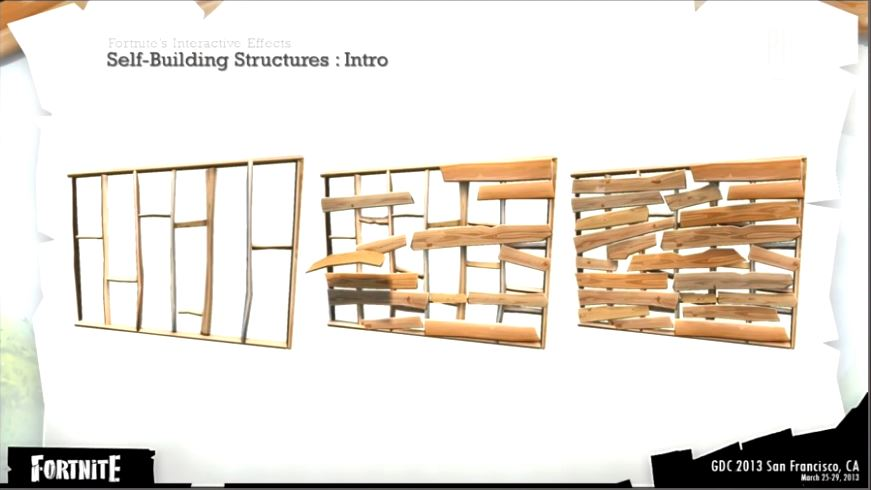
\includegraphics[scale=0.5]{wallimg.jpg}
  \caption{Wall block animation steps}
  \label{fig:wall}
\end{figure}

\section{Conclusion}
In conclusion, both vertex animation and skeletal animation have their strengths and weaknesses depending on the types of animations that need to be performed, so they should be used accordingly. Skeletal animations will most oftenly be the best used for specific or complex character animations, vertex animations will most oftenly be best used for animating environmental game objects or for animating special or simple effects for meshes.
\\~\\
But a note to be made is that skeletal animation can be quite costly performance wise, if you wanted to populate a game with many animated gameobjects or characters, skeletal animation might not be the way to do it, as the game engine would need to update a lot of joints, so coming up with creative ways of using vertex shaders (but not limited to vertex shaders) would be a good idea as they don't require updating bones/joints.
\\~\\
And to answer the question "when should Game Developers use Vertex Shader Animations over Skeletal Animations?", is that any time skeletal animation would be too costly on performance for a game to update a very high amount of joints/bones or if the animation required needs to animate the mesh in ways that isn't possible thought joint/bone manipulation, then vertex shader animations would be a very good alternative way to creating the needed animations. Or they might want to use Vertex shader animation alongside Skeletal animation to help with certain harder animation effects that can't be solely done through skeletal rigs.

\section{Show references}
\cite{one}\cite{two}\cite{three}\cite{four}\cite{five}\cite{six}\cite{seven}\cite{nine}\cite{ten}\cite{eleven}\cite{twelve}\cite{thirteen}
\bibliographystyle{ieeetran}
\bibliography{references}

\end{document}
